\chapter{Theoretical Framework}

Tyter. 

\section{Galaxy Clusters}
 
Glas.

dwarf stars contribute very little to the integrated light from an old stellar population (Smith 2015)

Galaxy clusters contain a population of stars gravitationally unbound to individual galaxies, yet still bound to the clusters overall gravitational potential, created by the stripping of stars from galaxies during interactions and mergers

\begin{figure}[H]
\centering
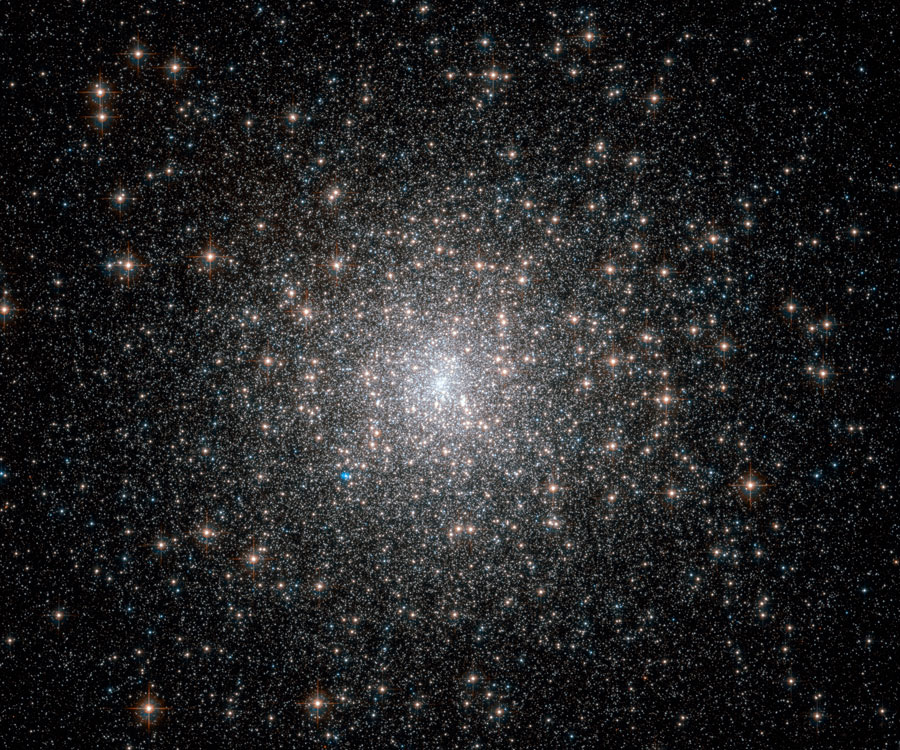
\includegraphics[width=12cm]{images/m15.jpg}
\caption[M]{G}
\end{figure}

T 

\begin{equation}
I(R)\sigma_{p}^{2}(R)=\frac{2}{\Gamma}\int_{R}^{\infty}\left(1-\beta\frac{R^{2}}{r^{2}}\right)\frac{\nu\bar{v_{r}^{2}}rdr}{\sqrt{r^{2}-R^{2}}}
\end{equation}

Whuster.  

\section{Gravitational Lensing}

\section{IMF in BCGs}



